\chapter{Results and Discussion} \label{ch:res}

In addition to the presented results in Sections \ref{ch:exp:results} and \ref{ch:sysid:case}, this chapter offers a holistic discussion on the outcome of this study, including the neural-network derived plant dynamics and the system identification of controllers. Section \ref{ch:res:interp} concerns the explainability of identified systems to classical control engineers and general users. Section \ref{ch:res:sim} presents the simulation of closed-loop system in MATLAB using modeled dynamics of each component. Section \ref{ch:res:lim} discusses the limitations of approaches employed by this study and encountered in the field of system identification at large. 

\section{Explainability} \label{ch:res:interp}

As neural network architectures and training data to be modeled become increasingly complex, researchers begin to emphasize the natural explainability of models for general users \cite{explainability1, explainability2}. In this work, the problem of explainability for the process dynamics model and the controller models is addressed through the lens of classical control theory using frequency analysis, specifically through bode plots, a graphical tool to characterize models by their frequency response. 

\subsection{Simulated Bode Plot of a Neural Network Model}

Traditionally, the analytical method of generating a bode plot is via obtaining the transfer function in the Laplace domain from the system's input to the desired output. However, this method loses its feasibility for black-box models including those derived from neural networks. Since developed models from machine learning and system identification approaches are able to make an inference on outputs from arbitrary input signals, simulated bode plots of the process dynamics are generated by making each of the four inputs (namely capstan speed, furnace power, helium temperature, and preform velocity) a sequence of sinusoidal signals of varying frequencies, while maintaining the other signals at their respective average value. For this analysis, the sinusoidal amplitude of each input signal is chosen to be the range of its typical fluctuation in production data, so that the inferred behavior closely resembles that in production. By logarithmically sampling the frequency space up to the Nyquist frequency\footnote{\emph{Nyquist frequency} is defined as half the sampling frequency, which, for the data in this study, is 1 Hz.}, as traditional bode plots do, the system's output signal is plotted in both time- and frequency- domain. Figure \ref{fig:bode_peak} illustrates the system response obtained via inference for one particular frequency; others exhibit similar behaviors. Due to the nonlinearity within the system, the output is not necessarily a single sinusoid; as the frequency-domain plot suggests, a sinusoidal input excites multiple higher frequencies in the system. Among all frequencies, we defined that a frequency is significant if its peak is greater than 5\% of the highest peak. A three-dimensional plot is generated depicting some of these significant frequencies\footnote{\label{ftn:sig}For graphical clarity, only the first 10 significant peaks were plotted for every input frequency.} excited by each input frequency and their respective FFT amplitudes. Refer to Figure \ref{fig:bode_3d}.

\begin{figure}[ht]
    \centering
    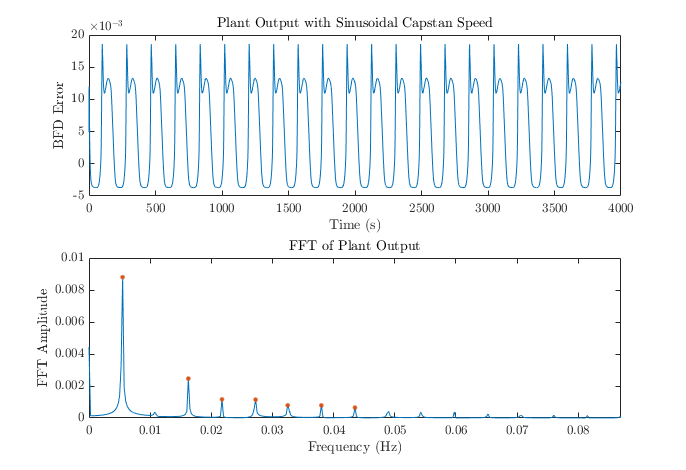
\includegraphics[width=\textwidth]{figures/bode_peak.png}
    \caption{Plant output with a sinusoidal capstan speed of typical amplitude (500 m/min) and frequency of 0.0054 Hz. The red dots mark the significant peaks as defined in Footnote \ref{ftn:sig} on the previous page.}
    \label{fig:bode_peak}
\end{figure}

It is evident that the dominant mode of each sinusoidal response is the one corresponding to the input frequency, shown in Figure \ref{fig:bode_3d} as the diagonal profile. Since the system is nonlinear, it is a common phenomenon that the gain (ratio of output amplitude to input amplitude) is a function dependent on the amplitude of the excitation. We can therefore generate simulated bode plots from each input to the BFD output, with input amplitudes sweeping across their typical ranges. The results of this analysis are shown in Figure \ref{fig:bode_profile}; they correspond to the diagonal profile of Figure \ref{fig:bode_3d} for different excitation amplitudes. It is noteworthy that, for some signals, such as the furnace power and the preform velocity, low-amplitude and high-amplitude inputs display different behaviors. The bifurcations of system behavior in different operational design domains is therefore graphically represented, and it is a smooth transition from one to another. 

\begin{figure}[hp]
    \centering
    \begin{subfigure}[b]{0.49\textwidth}
        \centering
        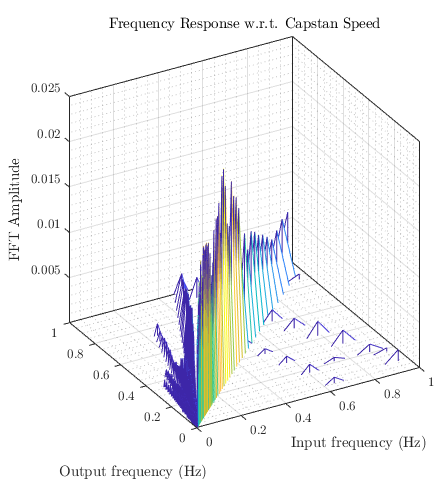
\includegraphics[width=\textwidth]{figures/bode_3d_1.png}
    \end{subfigure}
    \hfill
    \begin{subfigure}[b]{0.49\textwidth}
        \centering
        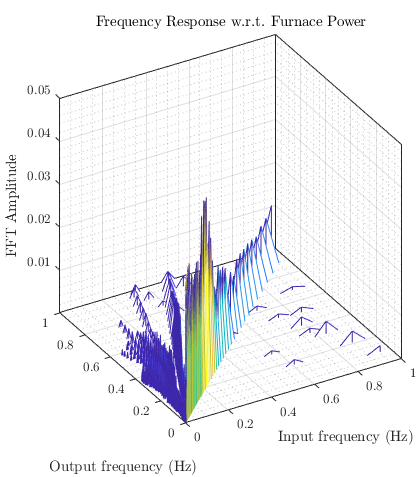
\includegraphics[width=\textwidth]{figures/bode_3d_2.png}
    \end{subfigure}
    
    \begin{subfigure}[b]{0.49\textwidth}
        \centering
        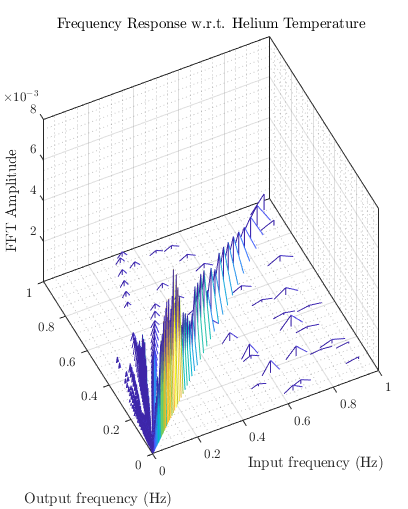
\includegraphics[width=\textwidth]{figures/bode_3d_3.png}
    \end{subfigure}
    \hfill
    \begin{subfigure}[b]{0.49\textwidth}
        \centering
        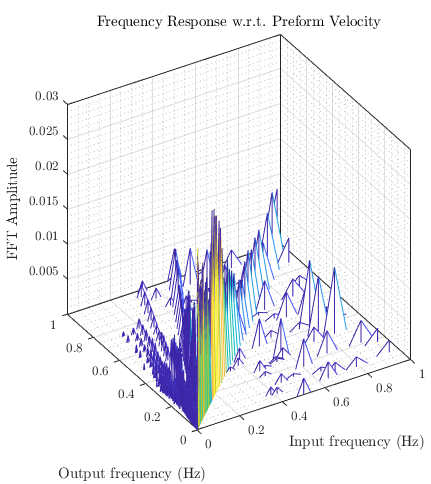
\includegraphics[width=\textwidth]{figures/bode_3d_4.png}
    \end{subfigure}
    
    \caption{3D plots illustrating high frequencies in the neural network plant model excited by sinusoids with a range of input frequencies.}
    \label{fig:bode_3d}
\end{figure}

\begin{figure}[ht]
    \centering
    \begin{subfigure}[b]{0.49\textwidth}
        \centering
        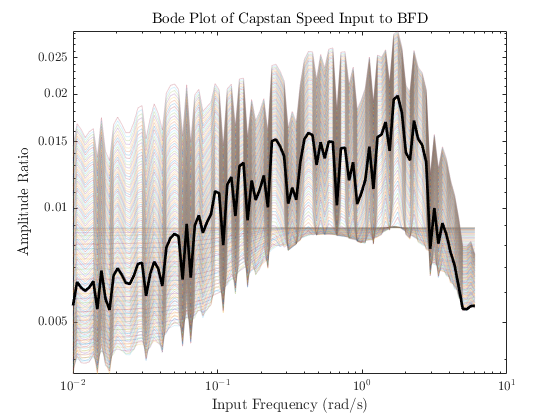
\includegraphics[width=\textwidth]{figures/bode_profile1.png}
    \end{subfigure}
    \hfill
    \begin{subfigure}[b]{0.49\textwidth}
        \centering
        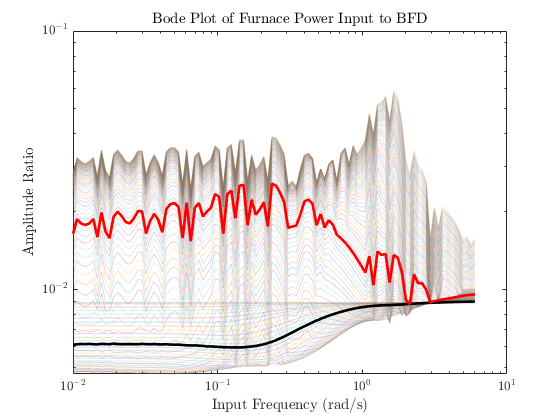
\includegraphics[width=\textwidth]{figures/bode_profile2.png}
    \end{subfigure}
    
    \begin{subfigure}[b]{0.49\textwidth}
        \centering
        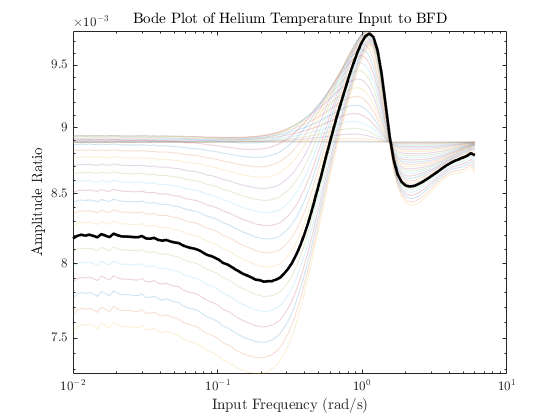
\includegraphics[width=\textwidth]{figures/bode_profile3.png}
    \end{subfigure}
    \hfill
    \begin{subfigure}[b]{0.49\textwidth}
        \centering
        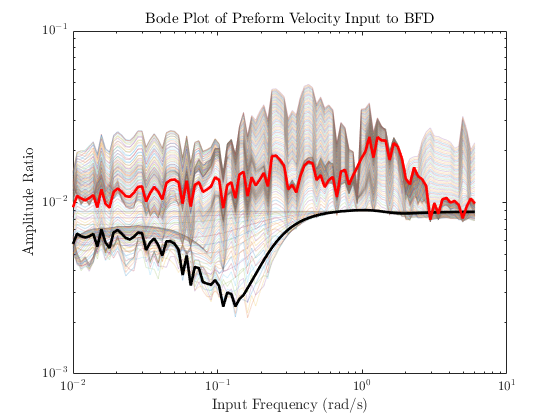
\includegraphics[width=\textwidth]{figures/bode_profile4.png}
    \end{subfigure}
    
    % \caption{Bode plots from each input to the BFD output. Note the variation as a function of excitation amplitudes, a characteristic phenomenon of nonlinear systems.}
    \caption{Bode plots from each input to the BFD output, corresponding to the diagonal profile in Figure \ref{fig:bode_3d}, for different excitation amplitudes. Note the bifurcation of system response for low and high amplitude inputs marked in red and black. }
    \label{fig:bode_profile}
\end{figure}

\subsection{Bode Plot of Subbatch Models to be Merged}

% need to write more ... ensemble model is representative of controller is by ... For instance, for the BFD controller, .... 
% maybe, "similarly for the tension controller, ..."
% change all to plurals

One way to confirm that the ensemble ARMAX model in Section \ref{ch:sysid:case} is representative of the BFD controller's behavior is by investigating the frequency response for each of the subbatch model. Figure \ref{fig:bode_armax_kd_kt} is the overlaid bode plot of the reasonably-fit subbatch models.\footnote{Bode plots depict the good subbatches from Tower 48 data.} All models have approximately equal roll-off rates within the mid- to high- frequency ranges. This consistency among subbatch models is further proven by the well-aligned exponential trend in the phase tending to high frequencies. The exponential drop in phase is attributed to the presence of input delay in the system, equivalently introducing an $e^{-s\Delta T}$ term in the transfer function, a linear factor that appears exponential when graphed logarithmically in the bode plot. ($\Delta T$ denotes the time delay.) This close agreement among the merged subbatch models proved the approach in obtaining the ensemble model reasonable. 

\begin{figure}[hp]
    \centering
    \begin{subfigure}[b]{0.9\textwidth}
        \centering
        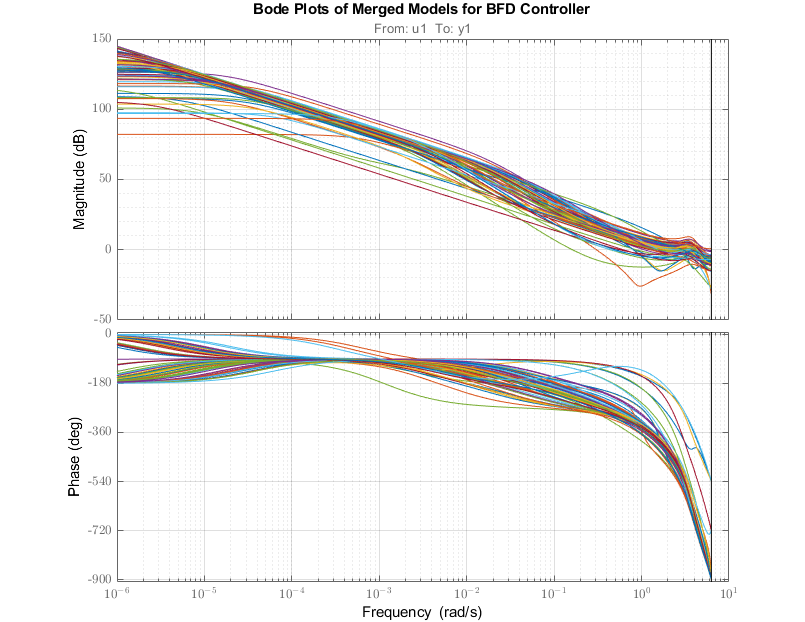
\includegraphics[width=\textwidth]{figures/bode_armax_kd.png}
    \end{subfigure}
    
    \begin{subfigure}[b]{0.9\textwidth}
        \centering
        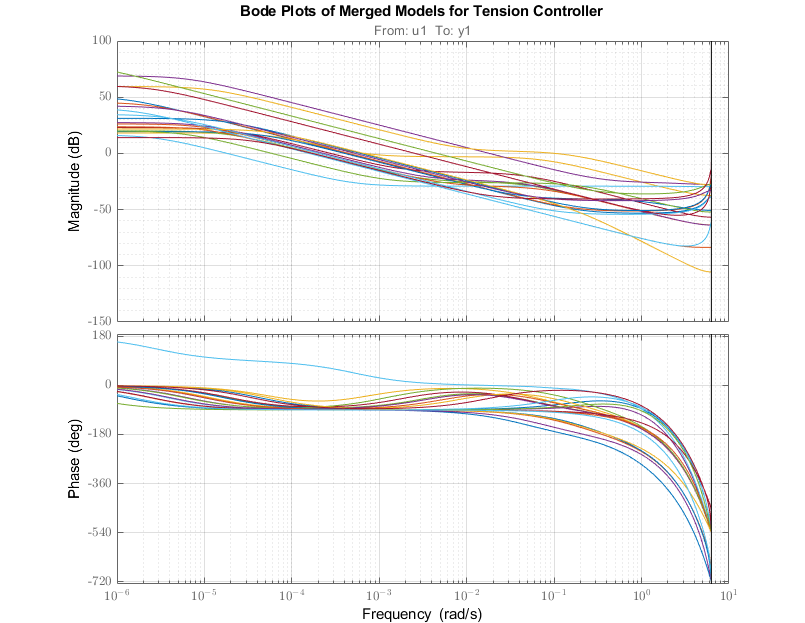
\includegraphics[width=\textwidth]{figures/bode_armax_kt.png}
    \end{subfigure}
    \caption{Aggregated bode plot of all subbatches to be merged into the ensemble ARMAX model.}
    \label{fig:bode_armax_kd_kt}
\end{figure}

\begin{figure}[ht!]
    \centering
    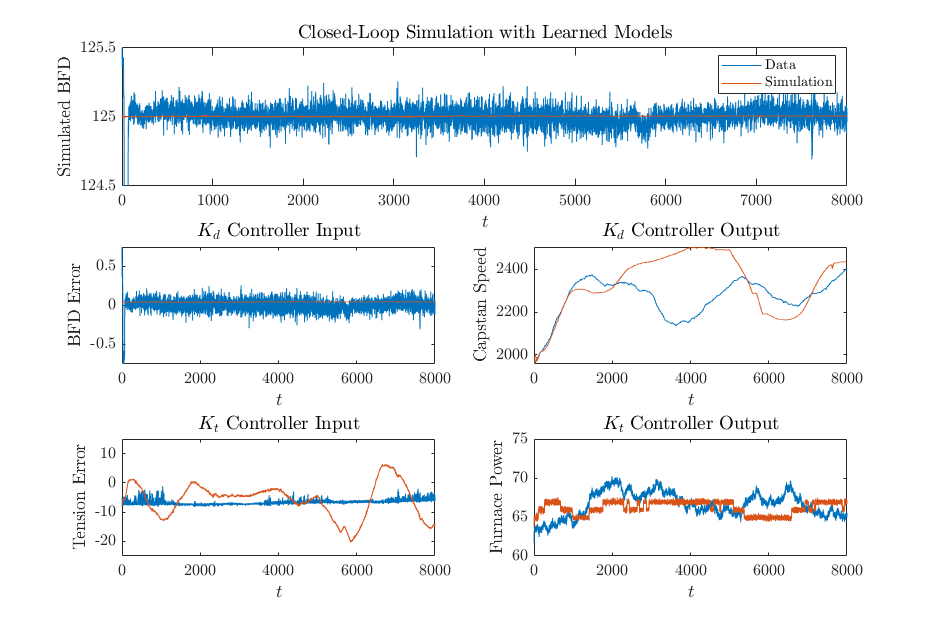
\includegraphics[width=\textwidth]{figures/closed_loop_simulation.png}
    \caption{Results of the closed-loop simulation on test data. Subplots contain important input and output signals and the predicted BFD by the neural network.}
    \label{fig:closed_loop_sim}
\end{figure}

\section{Closed-Loop Simulation} \label{ch:res:sim}

After developing surrogate models for the as-built process dynamics and controllers, the propagation of signals can be routed according to Figure \ref{fig:stl_system_diag} so that the closed-loop system outputs from identified models can be simulated. With the tension error and BFD error calculated from the feedback signal, the identified model of the BFD controller has an ARMAX structure given by 
\begin{equation}
    \begin{split}
        & y(t) + a_2y(t-1)+a_3y(t-2)+a_4y(t-3)+a_5y(t-4) \\ & = b_4u(t-3)+b_5u(t-4)+b_6u(t-5)+e(t)+c_2e(t-1)
    \end{split}
\end{equation}
Similarly the tension controller has a control law given by 
\begin{equation}
    \begin{split}
        & y(t) + a_2y(t-1)+a_3y(t-2)+a_4y(t-3) \\ & = b_4u(t-3)+b_5u(t-4)+e(t)+c_2e(t-1)+c_3e(t-2)
    \end{split}
\end{equation}
where all $a_i, b_i$ are parameters identified in procedures discussed in Section \ref{ch:sysid:case}. The output $y(t)$ of each signal can be then calculated and used as the input signal to the neural network, which predicts the tension and BFD outputs for the next timestep using the $\texttt{predictAndUpdateState}$ method in MATLAB. With specified BFD and tension setpoints, the closed-loop simulation is now able to simulate the learned controllers' behavior in maintaining these setpoints. The controller outputs then act as inputs to the neural network-derived aggregate plant to simulate the fiber drawing process. Figure \ref{fig:closed_loop_sim} shows this process for one particular subbatch of test data not used for training. This simulation is implemented in a MATLAB script. The source code for this closed-loop simulation and visualization is attached in Appendix \ref{apdx:code:sim}. The hyperlink to the GitHub repository for this study is also provided in the appendix.

\begin{figure}[ht!]
    \centering
    \begin{subfigure}[b]{\textwidth}
        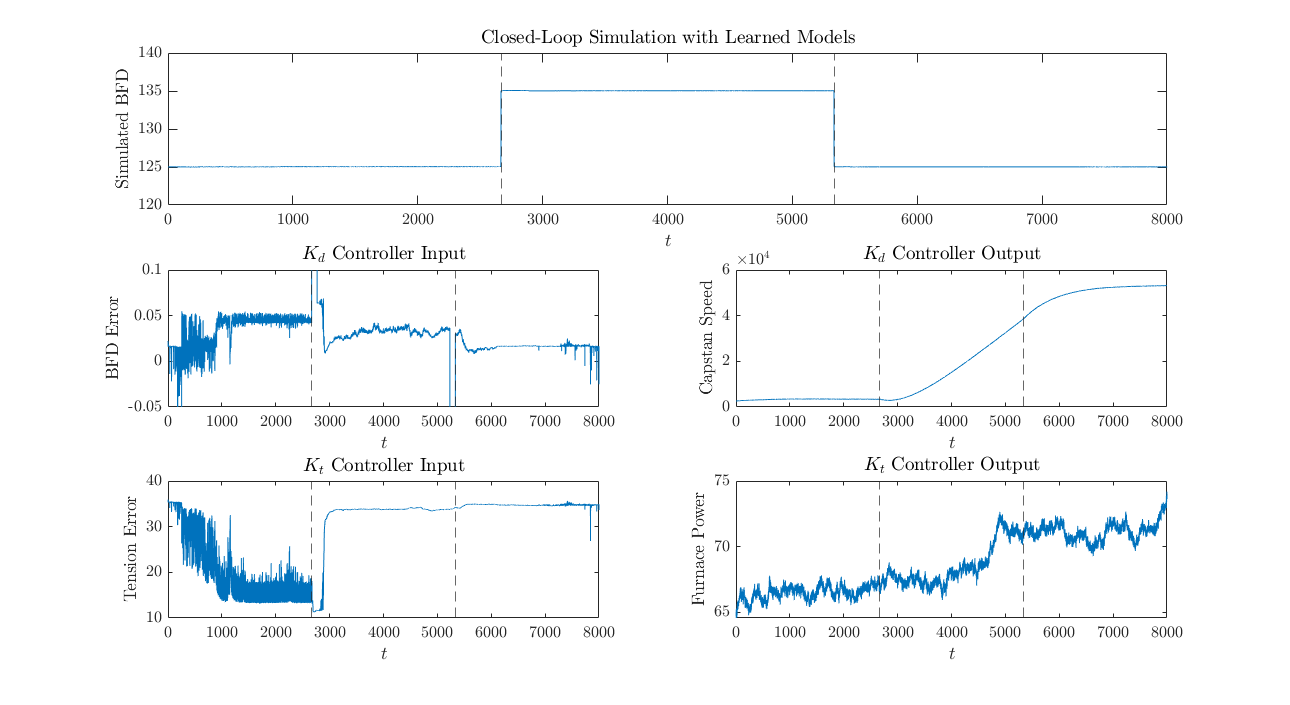
\includegraphics[width=\textwidth]{figures/closed_loop_sim_setpoint.png}
        \caption{Simulation with a change in BFD setpoint. Subfigures illustrate the transient behavior of controllers. }
        \label{fig:sim_setpoint}
    \end{subfigure}
    \begin{subfigure}[b]{0.48\textwidth}
        \centering
        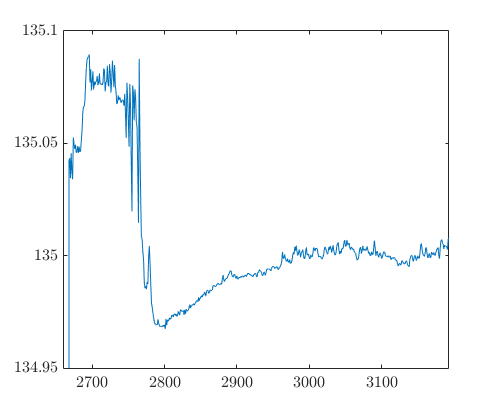
\includegraphics[width=\textwidth]{figures/setpoint_rising.png}
        \caption{Transient behavior on the rising edge of the setpoint change.}
    \end{subfigure}
    \hfill
    \begin{subfigure}[b]{0.48\textwidth}
        \centering
        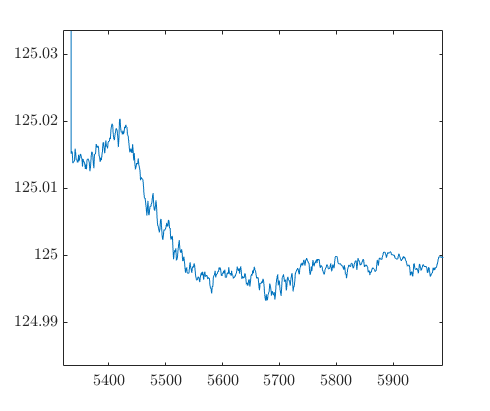
\includegraphics[width=\textwidth]{figures/setpoint_falling.png}
        \caption{Transient behavior on the falling edge of the setpoint change.}
    \end{subfigure}
\end{figure}

With this simulation as a design tool, a control engineer could visualize the system's transient behavior when there is a change in the setpoint. Figure \ref{fig:sim_setpoint} illustrates a hypothetical experiment in which the BFD setpoint changes from 125 to 135 then back to 125. 

There are profound implications of the controller deployment approach explored in this thesis. This approach builds on the models for the fiber drawing plant and controllers, augmented by first principle equations. With a learned model of the process dynamics and as-built controllers, simulations are built to replicate the system output and verify the accuracy and generalizability of the learned models. In this way, modifications to deployed industrial plants can be done first in simulation, which serves as a digital twin. The predicted output signals become reasonable heuristics to guide the controller improvement process. By defining related components as black-box systems, this study demonstrated that it is possible to identify these systems via machine learning and system identification techniques, integrate them and simulate a full as-built system. Further design improvements to the as-built system could be done first in simulation before implementing them for deployment. In doing so, the simulation serves not only as a digital twin to the hardware in production but also as a design tool for controller development and tuning.

In summary, the recommended procedure is as follows, 

\begin{enumerate}
    \item From data, obtain models for process dynamics, augmented with First Principles models
    \item From data, obtain models for as-built (aggregate) controllers 
    \item Simulate the as-built system with learned process models and as-built controllers
    \item Evaluate the closed-loop simulation, and demonstrate that it can replicate process data and modifications
    \item Use the process model to learn or improve the design of (potentially optimal) controllers 
    \item Simulate the new closed-loop system with improved controllers, evaluate system performance
    \item Deploy improved controllers, collect data, correct if necessary
\end{enumerate}

The approach is applicable to a versatile set of mechanical systems on which an extensive amount of data can be collected. Such examples include coffee roasters, food packaging assemblies, and robotic arms. 

\section{Limitations} \label{ch:res:lim}

The results above and in previous chapters successfully demonstrated the feasibility of this approach to model and simulate mechanical systems in production. Nevertheless, there are several limitations of this work I would like to acknowledge. These limitations stem from theoretical assumptions and inherent imperfections in hardware and in data. Tradeoffs must be made using engineering judgment to mitigate these issues. 

The theory behind autoregressive models like ARMAX assumes that the noise signal that enters the system is uncorrelated to the system's input signal. Many applications in real life cannot guarantee zero correlation. In particular, industrial plants with fast dynamics can have inputs that are more highly correlated with noise, whose frequency range may be similar to that of the process dynamics. Furthermore, parametric methods rely on the local linearization of the plant dynamics. The algorithm built upon linear time-invariant (LTI) systems succumbs to any nonlinearity exhibited by the plant. All the challenges discussed above could potentially lead to biased models for the system dynamics.

The quality of data is a major factor directly correlated with the learning accuracy. Hardware defects are one of the factors attributed to the compromised quality. The heated extrusion process is not perfectly insulated from the ambient environment, and the helium gas flow may have been turbulent in some collected data, which causes disturbance in the extrusion process and adds to the process noise. In addition, most of the data that the neural network was trained on reflected the process dynamics near steady-state, which may lead to an incomplete identified model. It is essential to excite the system with different input signals and initial conditions to obtain more complete data for system behavior. 

% if under control, does not poke the data in different directions, may not excite plants in many ways / modes … may be an incomplete model

Discrete sampling and quantization are additional factors that introduce errors in the data. As mentioned in Section \ref{ch:sysid:case}, the sampling time of the controllers is 100 milliseconds. However, due to the limited computing capacity onboard, the collected data were only logged every 500 milliseconds; the measurements in between were assumed to be zero-order hold. Measurements taken from various components of the plant come from different electrical boxes; the clock synchronization among all the sensors was not verified, either. It is not clear whether there is delay between measurements that were considered to have the same timestamp. Furthermore, sensors also have finite resolution, which is especially evident in the tension controller (e.g. Figure \ref{fig:kt_example}). If the actual value is between two adjacent quantized values, the output signal fluctuates between both values. 

Another shortcoming of sensors is that, as with any measured data from real-world experiments, measurement noise from sensors must be taken into account in data analysis. Visualizations in Chapter \ref{ch:sysid} already demonstrated that measured data are often corrupted by noise. (See Figures \ref{fig:bfd_input_output} and \ref{fig:kt_example}.) If the noise dynamics were modeled adequately, the system identification technique can better recover the underlying process dynamics from a noisy signal. However, the noise specifications of sensors on the plant happen to span a similar frequency range than high-frequency dynamics of the BFD, which we were interested in exploring. This added difficulty in achieving high accuracies using the system identification approaches. Noise also makes finite difference elements of the control loop highly susceptible to instability. % REFER TO LOOK UP TABLE 
The use of finite difference is also implicit in converting real systems to the general time-series model (refer to Equation \ref{eqn:pid_fd}). As claimed by Trischler et al., chaos can occur in one-dimensional finite-difference systems, in contrast to continuous differential equations where three dimensions are required \cite{trischler}.

% quality of data (coming from hardware defects - not insulated with ambient, sampling & quantization errors, clock not sync'ed, noisy sensors -> finite difference bad, chaos can occur in one-dimensional finite-difference systems, while three dimensions are required for chaos in continuous systems)
% noisy sensors - frequency specs overlaps with high freq dynamics, makes recovering original dynamics using sys id more difficult

There remain a few open challenges in developing purely data-based models for controllers. 

\begin{enumerate}
    \item Black-box models are data-hungry and data-specific. As mentioned above, the accuracy of a model depends on the hardware involved and the quality of measurement data. A low volume of data would also result in a high variance of the estimated parameters. %, the effect of which has been illustrated in Figure \ref{}. % CITE MODALITY PLOT
    An adequate model of a system should demonstrate good generalization capabilities on validation data. The combination of volume and specificity of the required data makes black-box system identification a challenging problem. 

    \item Striking a balance between performance and robustness is difficult. This has been the age-old question across the system identification, control, and machine learning communities, although referred to by different terms. An overly trained machine learning model is subject to \emph{overfitting}, which means its predictive performance degrades outside of training dataset it has seen. In system identification, a model of higher order may fit the input-output data to better accuracy, but it is difficult to justify with first principles and may face a similar problem with an overfitted model. Parameters within a controller must also be tuned to balance higher peak performance in specific scenario(s) vs. a more robust performance over a wider set of operational design domains \cite{tan_et_al}.
    % high order that fits well or low order ... ? % control - good in some ODD bad in others, machine learning - overfitting, RL -  trade-off. % QUOTE THE PAPER FROM THE TALK THE OTHER DAY (2022-03, SIM-TO-REAL LEARNING AGILE LOCOMOTION FOR QUADRUPED ROBOTS, TAN ET AL, 2018)
    
    \item From a classical controls perspective, controllers and systems identified by data-driven approaches (i.e. via neural networks and system identification techniques) may involve complex poles and zeros when analyzed in the Laplace domain. % CITE SOMETHING?
    It is also not straightforward as to how to further fine-tune them to optimize for custom specifications or specific frequency-related properties. 
    
    \item In many machine learning applications, the technique of \emph{transfer learning} has shown great promise \cite{transfer_learning_sdc, transfer_learning_cnn}. Weights and architectures from pre-trained models used almost directly, with some modifications, to solve similar problems. However, for controllers (especially in an established plant in production), the specificity of the plant and the lack of literature both may pose challenges in applying the transfer learning technique. 
\end{enumerate}

In fact, these open questions are not unique to this project. A large amount of literature (some cited above) also assessed each of these limitations in different applications. Section \ref{ch:concl:future_work} also details ways that some of these can be addressed in the future of this ongoing project. 